\documentclass{article}[12pt,a4paper]
\usepackage[utf8]{inputenc}
\usepackage{caption}
\usepackage{amsmath} 
\usepackage{hyperref}
\usepackage{csquotes}
\usepackage{graphicx}
\usepackage{listings }

\hypersetup{
    colorlinks=true,
    linkcolor=blue,
    filecolor=magenta,      
    urlcolor=cyan,
}

\title{Blast From The Past}
\author{Rátki Barnabás}
\date{2020.08.02}

\begin{document}
\maketitle

A probléma a következő volt:
\begin{displayquote}
Milyen Commodore-64 emulátorok vannak, és ezek közül melyik fut az ön gépén? (Egy elég!) Írjon ebben BASIC nyelvű programot, mely a felhasználótól bekér egy számot, majd a kapott számszor kiírja a NEPTUN kódját! Küldjön linket egy screenshotra, melyen az emulátorban látható a program, illetve a futtatás eredménye! (Segítség: https://www.c64-wiki.com/wiki/C64-Commands, illetve mindössze az INPUT, PRINT és FOR-TO-NEXT utasításokra van szükség. A beírt programot a RUN paranccsal lehet futtatni. Feltehető, hogy a user rendes számot ad meg, input validációval nem kell foglalkozni. Pro tip: lehet külső szerkesztőben (pl. Notepad) is írni a programot, majd innen illeszteni az emulátorba.)
\end{displayquote}

\section{Emulátor lista és választás}
A következő Commodore-64 emulátorok léteznek\footnote[1]{Forrás : \url{http://emulation.gametechwiki.com/index.php/Commodore_64_emulators}} : 
\begin{center}
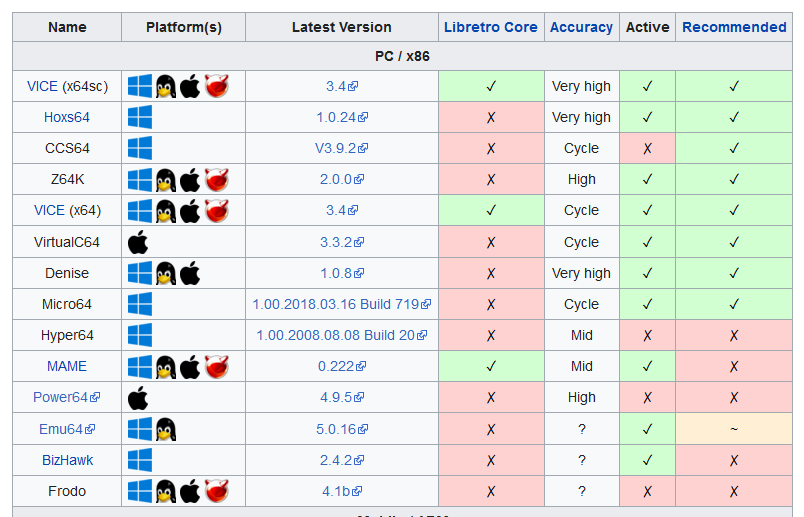
\includegraphics[scale=0.35]{graf1} 
\end{center}

A fentiek közül mindegyik kivéve \textit{VirtualC64} elfut a számítógépemen mivel Windows operációs rendszert használok. Ezek közül én a \textit{VICE} emulátort fogom használni a feladat megoldásához.

\section{Megoldás}
\begin{lstlisting}
10 input "hanysyor irja ki a kodjat:"; a%
20 for i=1 to a%: print "wpd2w5": next 
\end{lstlisting}
Ez a program a specifikált működést foglya produkálni, ennek bizonyítéka:
\begin{center}
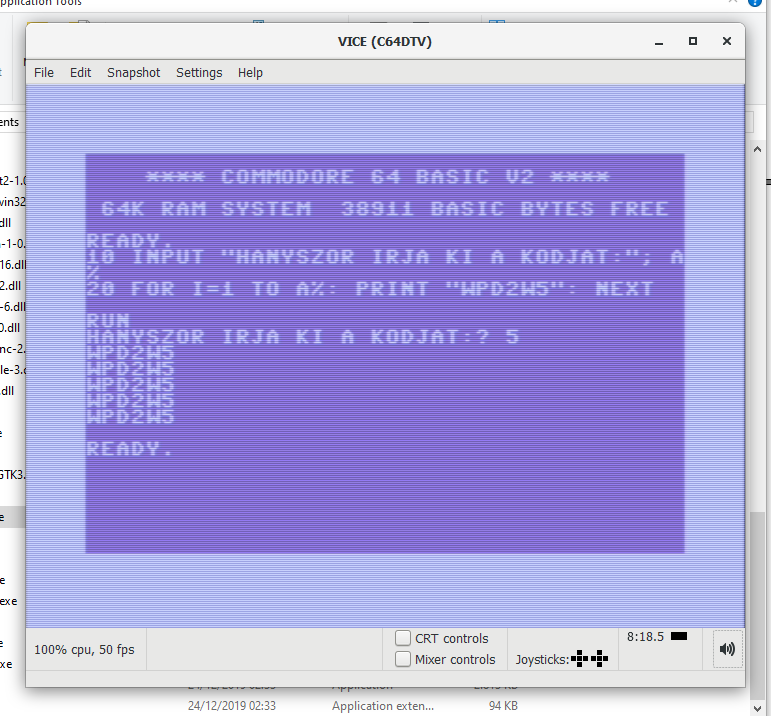
\includegraphics[scale=0.35]{graf2} 
\end{center}
\end{document}
